\section{What is an \ab{} workflow system?}

\subsection{What are \ab{} calculations?}

\begin{frame}{What are \ab{} calculations?}
    \begin{definitionblock}{\ab{} calculation}
        A method of calculating atomic and molecular structure directly from the first
        principles of quantum mechanics, without using quantities derived from experiment
        as parameters.
    \end{definitionblock}

    \begin{itemize}
        \item Electronic structure computation
        \item Optimize input crystal/molecular structures
        \item Phonon vibrational spectra computation
        \item Helmholtz free energy calculation at finite temperature
        \item Linear elastic constants
        \item More...
    \end{itemize}
\end{frame}

\begin{frame}{Typical \ab{} workflows used in our group}
    \begin{figure}[H]
        \centering
        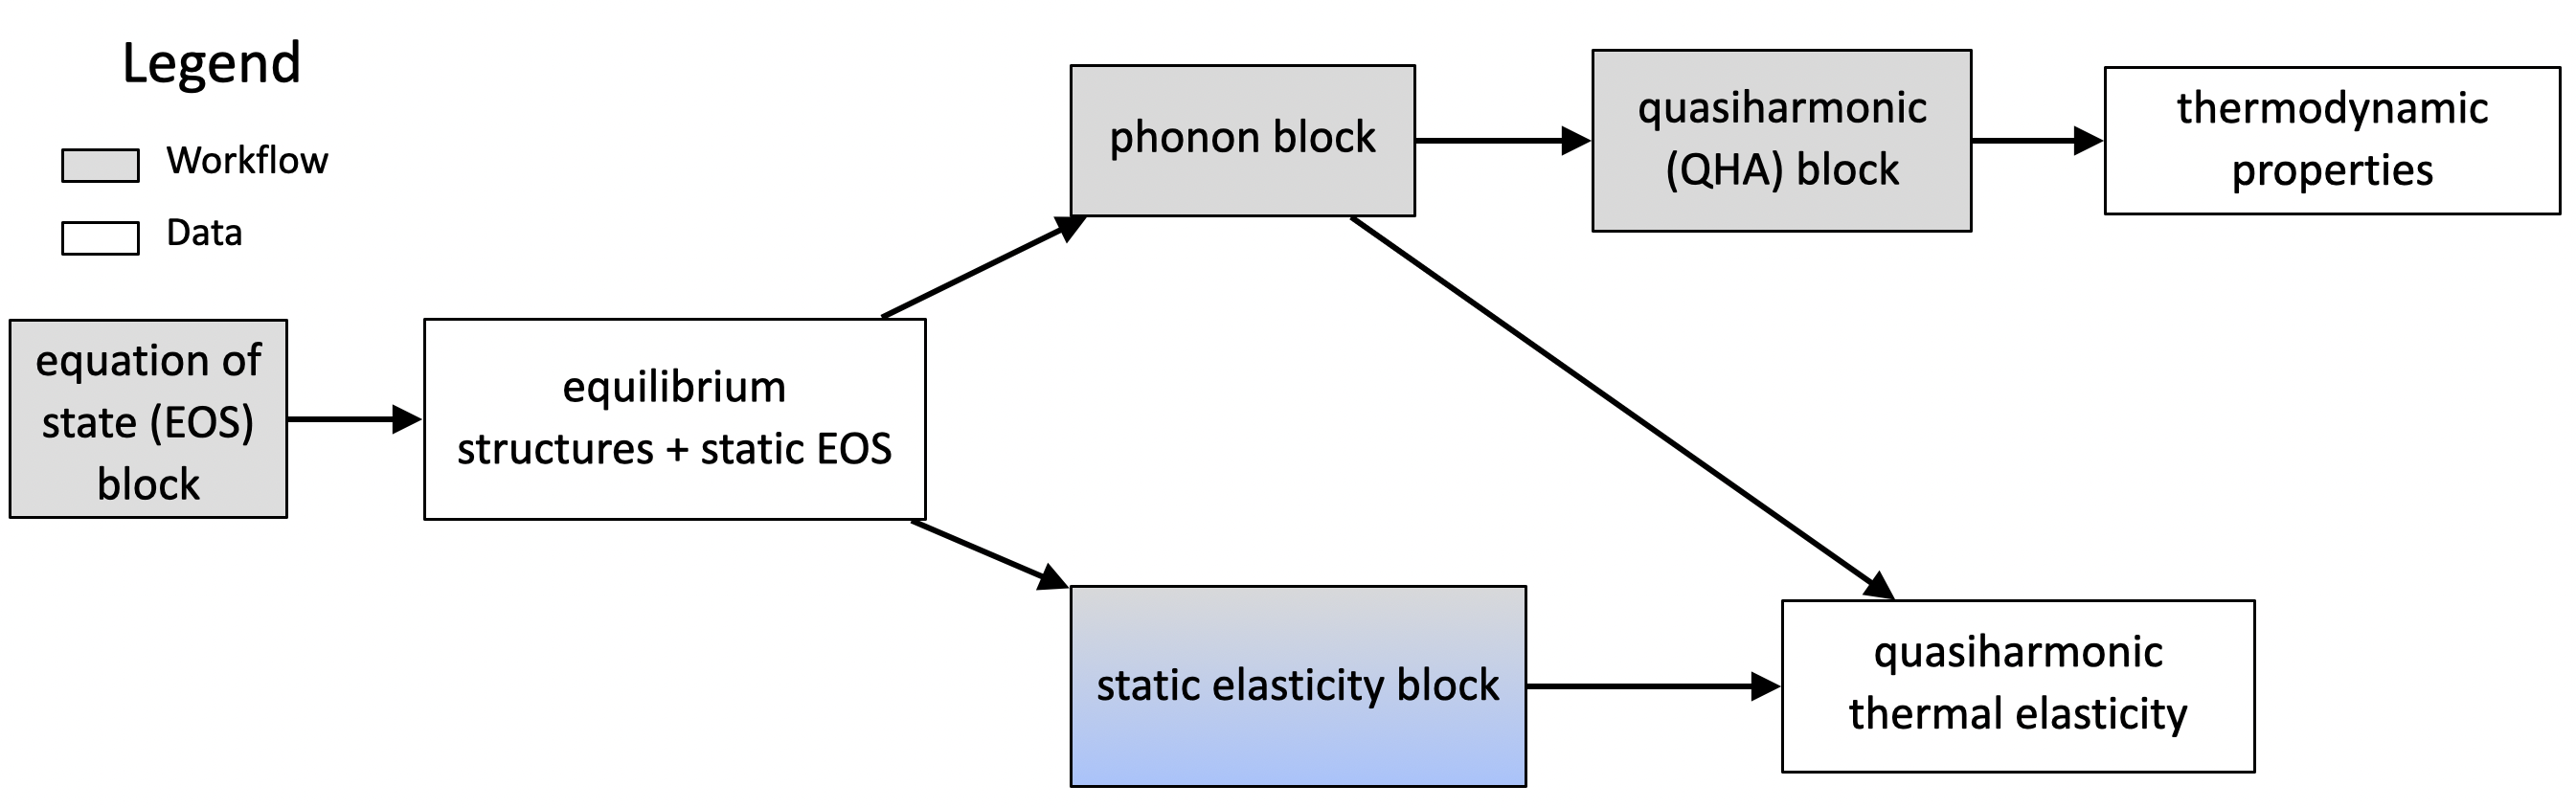
\includegraphics[height=0.4\textheight]{workflows}
        \label{eq:workflows}
    \end{figure}
\end{frame}

\subsection{What is needed in an \ab{} workflow system?}

\begin{frame}{What is needed in an \ab{} workflow system?}
    There are at least three components:

    \begin{itemize}
        \item Sciency, technical stuff: calculations, input generation, output analysis...
        \item Dispatcher, job scheduler: interacting with \ab{} software, \texttt{mpi}...
        \item User interface: interacting with users
    \end{itemize}
\end{frame}

\subsection{What does \express{} do?}

\begin{frame}{What does \express{} do?}
    A Julia-written
    \begin{itemize}
        \item extensible,
        \item lightweight,
        \item high-throughput,
        \item high-level
    \end{itemize}
    workflow framework that aims to automate \ab{} calculations for the materials science
    community.
\end{frame}
